\documentclass[a4paper]{article}
\usepackage[margin=1in]{geometry}%设置边距,符合Word设定
\usepackage{ctex}
\usepackage{setspace}
\usepackage{lipsum}
\usepackage{graphicx}%插入图片
\usepackage{cite}
\graphicspath{{Figures/}}%文章所用图片在当前目录下的 Figures目录

\usepackage{hyperref} % 对目录生成链接,注:该宏包可能与其他宏包冲突,故放在所有引用的宏包之后
\hypersetup{colorlinks = true,  % 将链接文字带颜色
	bookmarksopen = true, % 展开书签
	bookmarksnumbered = true, % 书签带章节编号
	pdftitle = 移动互联时代的营销变革, % 标题
	pdfauthor = 刘正浩} % 作者

\renewcommand{\contentsname}{\centerline{Contents}} %经过设置word格式后,将目录标题居中


\title{\heiti\zihao{2} 移动互联时代的营销变革}
\author{\songti 刘正浩 2019270103005}
\date{\today}


\begin{document}
	\maketitle
	\thispagestyle{empty}

\begin{abstract}
	从人类社会中诞生出商业开始,营销就是商业的一个重要组成部分。吆喝、响板、牌匾,都是古代中国的人们进行营销的例子。
	进入现代社会之后,营销手段与古代相比有了很大的不同。不同传媒工具(如电话、电视等)的诞生,催生出了电话催销、电视广告等等新兴的营销方式。
	而手机、平板电脑等移动通信终端的发展,又催生出了一个新的营销方式:基于移动互联网的营销。由于手机、平板电脑等移动通信终端的出现几乎影响到了每个人生活的方方面面,
	可以说,移动互联网对营销方式、营销手段的改变也是深刻的。
\end{abstract}

\tableofcontents
\newpage

\section{背景}
	\subsection{移动互联网}
		\begin{figure}[htbp]
			\centering
			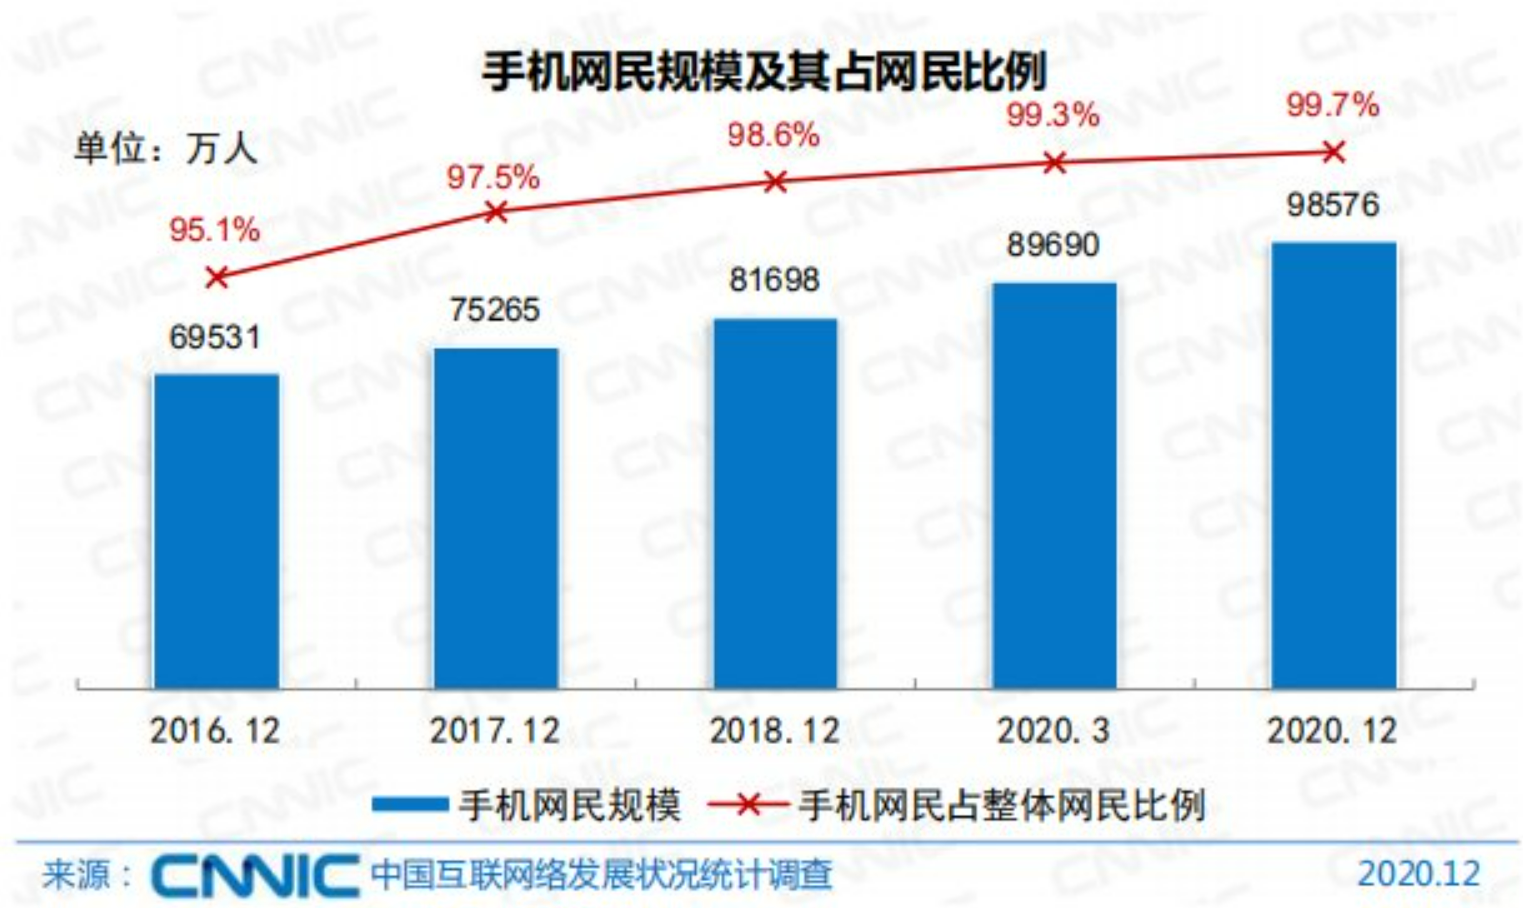
\includegraphics[scale=0.25]{1.png}
			\caption{手机网民规模及其占网民总数比例}
		\end{figure}
		实际上,移动互联网只是互联网的一部分,它是传统PC互联网的延续、继承与延伸。它延续了传统PC互联网的技术手段、继承了传统PC互联网的诸多特性,所以基于移动互联网的营销与传统的网络营销具有许多相似的地方。
		但移动互联网也与传统PC互联网有着很明显的不同——移动互联网有着移动的特性。正因为这个特性,移动互联网比PC互联网离我们每个人的距离都更近,也更容易融合进我们的日常生活中,更加深刻地改变了我们的生活方式。
		根据中国互联网络信息中心(CNNIC)发布的第47次《中国互联网络发展状况统计报告》,在2020年12月时,我国的手机网民规模已经超过了9.8亿,占网民总数比例超过99.7\%。(如图1)
		可见,利用移动互联网广泛而又贴近生活的特性进行营销活动是自然而又很有必要的。拥有如此庞大规模的移动互联网正不断催生出新的业态、新的营销方式,
		也有许多学术机构和企业不断研究这些新型的营销方式并创造出更新的营销方式。可以说,移动互联网是一个催生出不同营销方式的大“温室”。
		

\section{基于移动互联网的营销的特征与优势}
	2011年,美国人约翰·杜尔将互联网的三个关键词Social(社交)、Local(地域)和Mobile(移动)结合在一起,提出了基于移动互联网的营销SoLoMo概念。
	其中,Social指的是移动互联网营销的社会性,即移动互联网的形成需要网民的互相连接,同时,这些网民可能会形成或大或小的社群,这些不同的社群是在营销过程中需要进行考虑的用户群体的重要形式之一;
	Local指的是移动互联网营销的地域性,即移动互联网营销要以目标消费者的地理位置为基础;Mobile指的是移动互联网营销需要基于稳定、成熟的移动互联网技术来进行活动。
	在SoLoMo框架中,企业营销是以社交化的网民连接(Social)为基础,消费者利用移动互联网和移动终端(Mobile),企业结合消费者地理信息(Local),让消费者可以随时随地进行商品信息的收集、比较、分析和决策,
	从而方便消费者购买商品。\cite{1}
	由于移动互联网相较于传统互联网具有高效、精准、编写、低成本、个性化、无处不在的特性,因而基于移动互联网的营销也具有很鲜明的特征:营销信息更加贴合消费者个人喜好、信息更生动、成本更低廉、及时性更好等等。
	在移动互联网环境下,商家与消费者之间的互动相较于传统营销方式有显著的增加:商家可以向顾客发送即时、直接、个性化精准定位的商品信息以招揽到更多顾客,顾客也可以在第一时间联系到商家,更加快速、便捷地完成交易过程或者解决在交易过程中产生的问题。
	同时,基于顾客的位置信息,商家还可以随着消费者的位置变化提供针对性强的相应产品或者服务推荐,可以做到在对的时间、对的地点为消费者提供需要的商品或服务信息。

\section{移动互联网营销的主要技术手段}
	实际上,移动互联网营销所依靠的技术手段之一是一个近年来非常火爆的名词——大数据。大数据脱胎于“数据”,但它由于传统意义上的数据有着很显著的区别。
	大数据的“大”,将它与传统数据的区别完全地展现了出来。传统的计算机或者服务器产生的数据可能在GB(1GB=$2^{30}$字节;字节是计算机存储数据的最小单位,大小为八位二进制数,如10011010)甚至TB(1TB=1024GB)数量级,
	而大数据的大小可能能达到EB($2^{60}$字节)量级,由此可见大数据的规模有多大。
	虽然许多人把大数据吹得神乎其神,甚至出现了“大数据算命”这一令人哭笑不得的噱头,但实际上,目前大多数企业利用大数据的原理非常简单:用海量的数据结合已有的数学模型来尽可能精准地刻画出一个对象的不同特征。在营销中,它就体现为刻画用户(消费者)
	形象的“用户画像”这一过程。有了用户画像,企业就可以针对具有不同画像的用户展开特别的营销。\par
	具体到营销体系的各个环节,不同的机构也已经开始基于全媒体营销以及大数据处理带来的新要求,获得了新的发展空间。一方面,大数据对于营销体系中的相关机构提出了全新的要求,对于数据服务公司来说,需要能够掌握实时、海量的数据检测技术,
	具备构建大数据挖掘模型的能力,增强大数据分析能力; 对于媒体机构来说则需要能够记录信息痕迹,建立海量数据库,能够运用大数据分析和优化自身的内容、产品与营销服务; 对于广告营销机构来说,则需要能够以多样化的手段追踪广告效果,
	应用大数据分析媒体的广告价值,优化广告营销服务; 对于第三方技术公司来说,则需要能够提供大数据的采集、存储和分析的技术支撑,同时提供大数据挖掘技术的解决方案。总的来说,数据挖掘能力和应用能力是全媒体营销时代必备的能力。\par
	另一方面,在适应了新时代的营销要求之后,这些机构也逐步通过大数据提升自身的营销价值。例如,目前世界最大的社交网站 Facebook 利用用户的基本属性、粉丝、兴趣来找出潜在的用户群,基于这样的广告模式,
	Facebook 的广告投放系统也基本上以自助式为主。自助广告投放先由自定义受众开始。Facebook 提供三种方式: 第一,使用11个维度的人口统计特征来定义受众的基本属性; 第二,根据粉丝页进行筛选; 第三,根据用户设定的兴趣进行筛选,
	然后,广告主需要提交广告活动的总预算和每天的预算额。系统会根据广告主设定的受众条件,运算出目标受众群的人数,然后根据广告主选择的广告方式 (CPM/CPC) 给出建议费用的范围。通过后台数据,广告主可以在广告投放系统上了解数据动态,随时更改策略。
	\cite{2}
\section{移动互联网营销与传统营销的区别}
	基于移动互联网的营销与传统的营销之间有着很大的区别。\par
	首先,基于移动互联网的营销的信息源相较于传统营销而言更加广泛。以投放广告为例,传统营销投放的广告主要以电视、广播、报纸等作为媒介,而移动互联网营销投放的广告以在手机APP中投放的广告为主。
	由于电视、广播与报纸相较于手机APP而言与客户的日常生活更远,而手机APP不受时间、地点的限制,所以在手机APP中投放广告,吸引到顾客的效率要比电视、广播和报纸要高。\par
	其次,用户获取信息的方式更加主动。用户在看报纸、听广播时,进行的主要活动是接收信息,即“报纸上有什么,用户就只能看到什么”,这样的信息获取方式是被动的。
	由于用户只能看到电视或报纸上刊登的广告,他们所能接触到的商品信息是少量的。相反,手机APP给予用户充足的选择权,他们可以借助手机看到市面上的几乎一切商品,这样的信息获取方式是主动而广泛的。
	相应地,用户接受营销信息的机会也更加广泛,这样就能给商家或者企业提供更大的营销空间。\par
	另外,移动互联网媒介的社交性大大增加。在许多手机APP中都会形成或大或小的用户社群,这些用户社群内部具有一定的互动频率和相似的用户画像,针对这些不同用户社群单独进行营销也是目前企业营销的重要手段之一。
	移动互联网的社交性让营销不再是简单的企业-消费者这一方向,在消费者之间会有更加明显的对某某企业的“评价”说法,也就是口碑形成更加快速和深刻。只有更加认真地保持好口碑,才可能在移动互联网时代真正做好一个企业。
\bibliographystyle{plain}% 参考文献引用格式
\bibliography{books}
\end{document}